\documentclass[10pt]{report}

\usepackage{stan-talks}

\begin{document}
\sf
\vspace*{6pt}
\noindent
\spc{\huge\bfseries \color{MidnightBlue}{Section 2.}
\\[8pt]
\spc{\Huge\bfseries \color{MidnightBlue}{Stan Components}}}
\vfill
\noindent
\spc{\large\bfseries Bob Carpenter}
\\[4pt]
\spc{Columbia University}
\vfill
\hfill 

\mypart{Part I}{Stan Top Level}

\sld{Stan's Namesake}
\begin{itemize}
\item Stanislaw Ulam (1909--1984)
\item Co-inventor of Monte Carlo method (and hydrogen bomb)
\item[]
  \begin{center}
    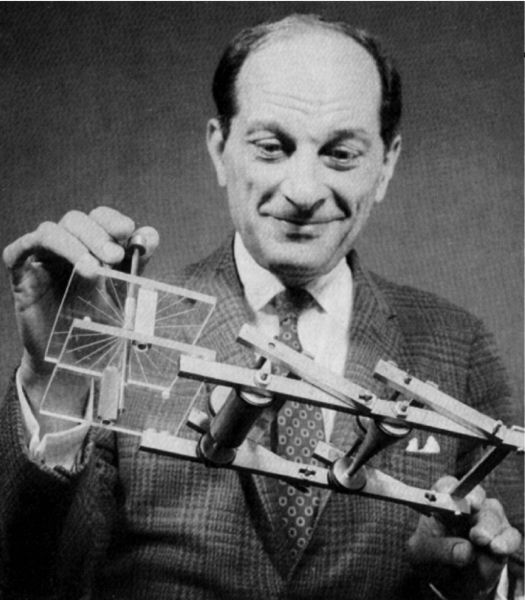
\includegraphics[width=0.25\textwidth]{img/ulam-fermiac.jpg}
  \end{center}
  {\small
  \item Ulam holding the Fermiac, Enrico Fermi's physical Monte Carlo simulator
    for random neutron diffusion}
\end{itemize}

\sld{What is Stan?}
\begin{itemize}
\item Stan is an \myemph{imperative} probabilistic programming language
\vspace*{-12pt}
  \begin{subitemize}
  \item  cf., BUGS: declarative; \ Church: functional; \ Figaro: object-oriented
  \end{subitemize}
\item Stan \myemph{program}
  \begin{subitemize}
  \item declares data and (constrained) parameter variables
  \item defines log posterior (or penalized likelihood)
  \end{subitemize}
\item Stan \myemph{inference}
  \begin{subitemize}
  \item MCMC for full Bayesian inference
  \item VB for approximate Bayesian inference
  \item MLE for penalized maximum likelihood estimation
  \end{subitemize}
\end{itemize}

\sld{Platforms and Interfaces}
\vspace*{-2pt}
\begin{itemize}
\item \myemph{Platforms}:  Linux, Mac OS X, Windows
\item \myemph{C++ API}: {\small portable, standards compliant (C++03)}
\item \myemph{Interfaces}
  \begin{subitemize}\footnotesize
  \item \myemph{CmdStan}: Command-line or shell interface (direct executable)
  \item \myemph{RStan}: R interface (Rcpp in memory)
  \item \myemph{PyStan}: Python interface (Cython in memory)
  \item \myemph{MatlabStan}: MATLAB interface (external process)
  \item \myemph{Stan.jl}: Julia interface (external process)
  \item \myemph{StataStan}: Stata interface (external process)
      [under testing]
    \end{subitemize}
\item \myemph{Posterior Visualization \& Exploration}
\begin{subitemize}
 \item \myemph{ShinyStan}: Shiny (R) web-based
\end{subitemize}
\end{itemize}
\vfill


\sld{Who's Using Stan?}
\begin{itemize}
\item 1200 \myemph{users group} registrations;  10,000 manual
  \myemph{downloads} (2.5.0); 300 Google scholar citations (100+ fitting)
\item \myemph{Biological sciences}: {\footnotesize
clinical drug trials, entomology, opthalmology,
neurology, genomics, agriculture, botany, fisheries,
cancer biology, epidemiology, population ecology, neurology
}
\item \myemph{Physical sciences}: {\footnotesize 
astrophysics, molecular biology, oceanography, climatology
}
\item \myemph{Social sciences}: {\footnotesize
 population dynamics, psycholinguistics, social networks, political science
}
\item \myemph{Other}: {\footnotesize materials engineering, finance, actuarial,
  sports, public health, recommender systems, educational testing}
\end{itemize}

\sld{Documentation}
% 
\begin{itemize}
\item {\slshape Stan User's Guide and Reference Manual}
\begin{subitemize}
\item 500+ pages
\item Example models, modeling and programming advice
\item Introduction to Bayesian and frequentist statistics 
\item Complete language specification and execution guide
\item Descriptions of algorithms (NUTS, R-hat, n\_eff)
\item Guide to built-in distributions and functions
\end{subitemize}
\item Installation and getting started manuals by interface
\begin{subitemize}
\item RStan, PyStan, CmdStan, MatlabStan, Stan.jl
\item RStan vignette
\end{subitemize}
\end{itemize}

\sld{Books and Model Sets}
\begin{itemize}
\item \myemph{Model Sets} Translated to Stan
\begin{subitemize}
\item BUGS and JAGS examples (most of all 3 volumes) 
\item Gelman and Hill (2009) {\slshape Data Analysis Using Regression and
    Multilevel/Hierarchical Models}
\item Wagenmakers and Lee (2014) {\slshape Bayesian Cognitive Modeling}
\end{subitemize}
\item \myemph{Books} with Sections on Stan
\begin{subitemize}
\item Gelman et al. (2013) {\slshape Bayesian Data Analysis}, 3rd Edition.
\item Kruschke (2014) {\slshape Doing Bayesian Data Analysis, Second
    Edition: A Tutorial with R, JAGS, and Stan}
\item Korner-Nievergelt et al. (2015) {\slshape Bayesian Data Analysis in
    Ecology Using Linear Models with R, BUGS, and Stan}
\end{subitemize}
\end{itemize}

\sld{Scaling and Evaluation}
\begin{center}
\vspace*{-6pt}
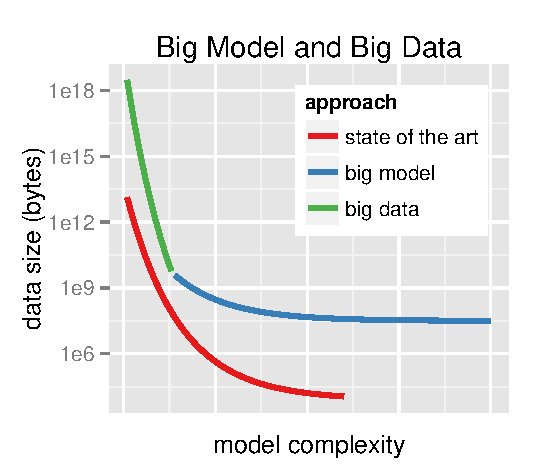
\includegraphics[width=0.4\textwidth]{img/big-model-big-data.pdf}
\vspace*{-6pt}
\end{center}
\begin{itemize}
\item Types of Scaling: data, parameters, \myemph{models}
\item Time to converge and per effective sample size: \\[2pt]
\mbox{ } \ \ \ {0.5--{\large$\infty$} times faster than BUGS \& JAGS}
\item Memory usage: \ {1--10\% of BUGS \& JAGS}
\end{itemize}


\sld{NUTS vs.\ Gibbs and Metropolis}

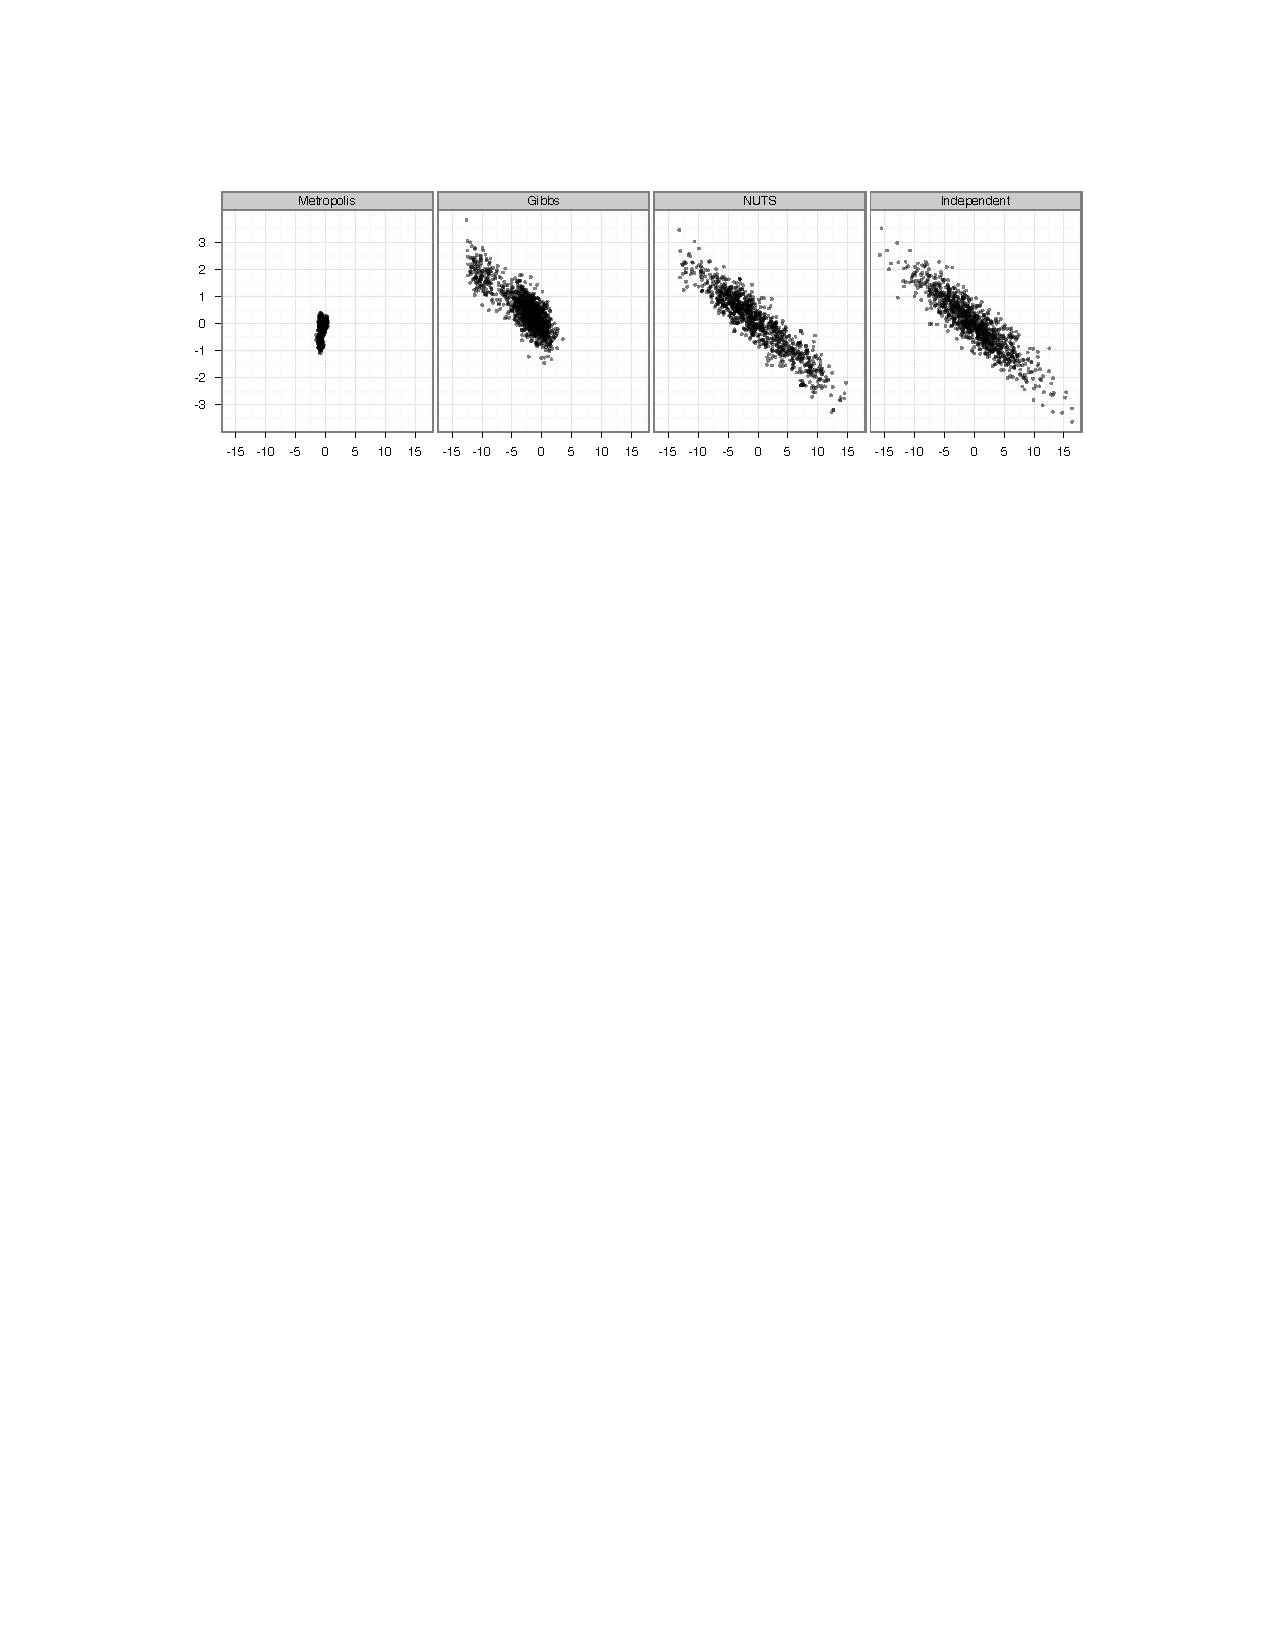
\includegraphics[width=0.9\textwidth]{img/nuts-vs.pdf}
\begin{subitemize}
\item Two dimensions of highly correlated 250-dim normal
\item \myemph{1,000,000 draws} from Metropolis and Gibbs (thin to 1000)
\item \myemph{1000 draws} from NUTS; 1000 independent draws
\end{subitemize}

\sld{Stan's Autodiff vs.\ Alternatives}

\begin{subitemize}
\item Among \myemph{C++ open-source} offerings: 
Stan is \myemph{fastest} (for gradients), 
\myemph{most general} (functions supported), 
and \myemph{most easily extensible} (simple OO)
\end{subitemize}
\vspace*{-8pt}
\hfill
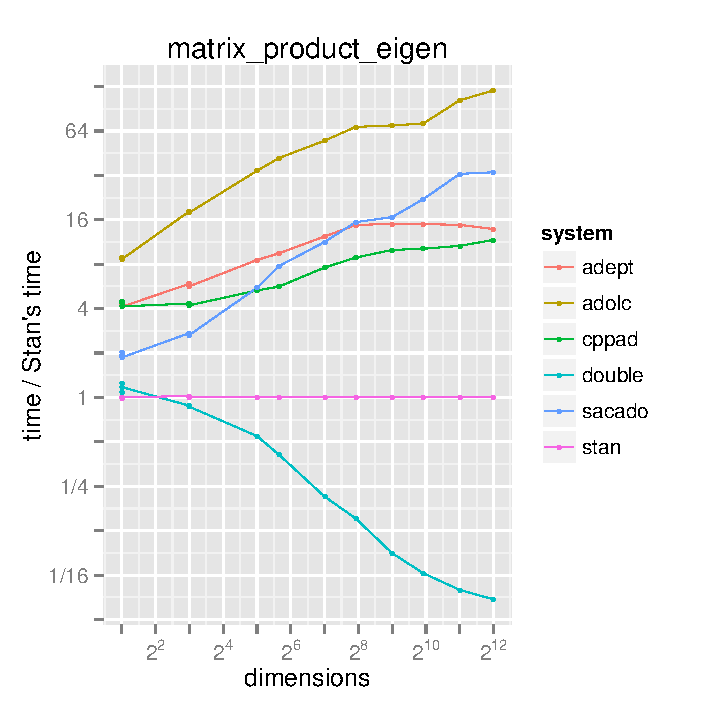
\includegraphics[width=0.45\textwidth]{img/autodiff-eval-matrix-product-eigen.pdf}
\hfill
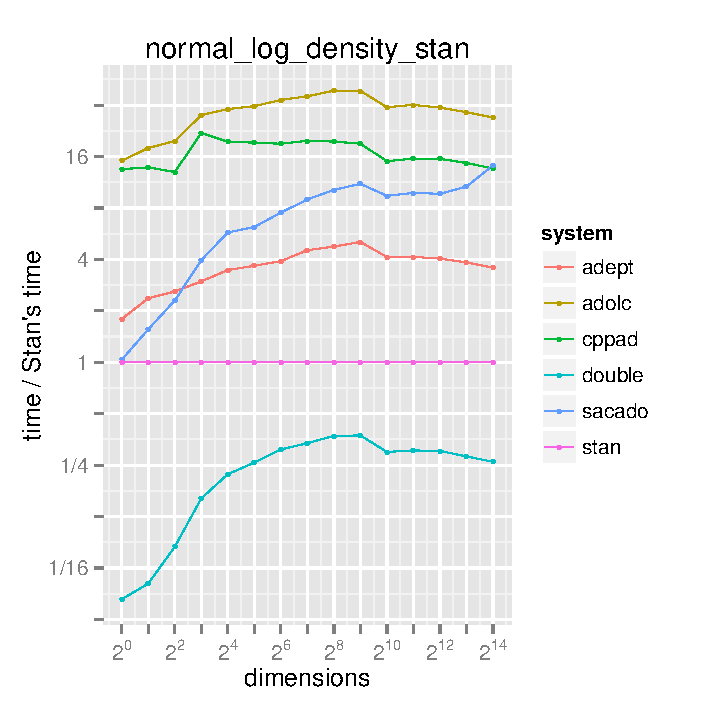
\includegraphics[width=0.45\textwidth]{img/autodiff-eval-normal-density.pdf}
\hfill


\mypart{Part II}{Stan Language}

\sld{Stan is a Programming Language}
\begin{itemize}
\item \myemph{Not} a graphical specification language like BUGS or JAGS
\item Stan is a Turing-complete imperative programming langauge for specifying differentiable log densities
\begin{subitemize}
\item reassignable local variables and scoping
\item full conditionals and loops
\item functions (including recursion)
\end{subitemize}
\item With automatic ``black-box'' inference on top (though even that is tunable)
\item Programs computing same thing may have different efficiency
\end{itemize}


\sld{Basic Program Blocks}

\begin{itemize}
\item \myemph{\tt\bfseries data} \ (once) 
  \vspace*{-4pt}
  \begin{itemize}\small
  \item {\slshape content}: declare data types, sizes, and constraints
  \item {\slshape execute}: read from data source, validate constraints
  \end{itemize}
  % 
\item \myemph{\tt\bfseries parameters} \ (every log prob eval)
  \vspace*{-4pt}
  \begin{itemize}\small
  \item {\slshape content}: declare parameter types, sizes, and constraints
  \item {\slshape execute}: transform to constrained, Jacobian
  \end{itemize}
  % 
\item \myemph{\tt\bfseries model} \ (every log prob eval) 
  \vspace*{-4pt}
  \begin{itemize}\small
  \item {\slshape content}: statements definining posterior density
  \item {\slshape execute}: execute statements
  \end{itemize}
\end{itemize}

\sld{Derived Variable Blocks}

\begin{itemize}
\item \myemph{\tt\bfseries transformed data} (once after data)
  \vspace*{-4pt}
  \begin{itemize}\small
  \item {\slshape content}: declare and define transformed data variables
  \item {\slshape execute}: execute definition statements, validate constraints
  \end{itemize}
  % 
\item \myemph{\tt\bfseries transformed parameters} (every log prob eval)
  \vspace*{-4pt}
  \begin{itemize}\small
  \item {\slshape content}: declare and define transformed parameter vars
  \item {\slshape execute}: execute definition statements, validate constraints
  \end{itemize}
  % 
\item \myemph{\tt\bfseries generated quantities} (once per draw, 
  \code{double} type)
  \vspace*{-4pt}
  \begin{itemize}\small
  \item {\slshape content}: declare and define generated quantity
    variables; \\
    includes pseudo-random number generators
    \\
    {\footnotesize (for posterior predictions, event probabilities,
      decision making)}
  \item {\slshape execute}: execute definition statements, validate constraints
  \end{itemize}
  % 
\end{itemize}


\sld{Variable and Expression Types}
\\[3pt]
\hspace*{17pt}Variables and expressions are \myemph{strongly, statically typed}.
\begin{itemize}
\item \myemph{Primitive}: {\tt\small int}, \ {\tt\small real}
\item \myemph{Matrix}: {\tt\small matrix[M,N]}, \ {\tt\small vector[M]}, \ {\tt\small row\_vector[N]}
\item \myemph{Bounded}: primitive or matrix, with 
  \\ {\tt\small <lower=L>}, \ {\tt\small <upper=U>}, \ {\tt\small <lower=L,upper=U>}
\item \myemph{Constrained Vectors}: {\tt\small simplex[K]}, \ {\tt\small
    ordered[N]},
  \\ {\tt\small positive\_ordered[N]}, \ {\tt\small unit\_length[N]}
\item \myemph{Constrained Matrices}: {\tt\small cov\_matrix[K]}, \ {\tt\small
    corr\_matrix[K]}, \ {\tt\small cholesky\_factor\_cov[M,N]}, \
  {\tt\small cholesky\_factor\_corr[K]}
\item \myemph{Arrays:}  of any type (and dimensionality)
\end{itemize}

\sld{Integers vs. Reals}
\begin{itemize}
\item Different types (conflated in BUGS, JAGS, and R)
\item Distributions and assignments care
\item Integers may be assigned to reals but not vice-versa
\item Reals have not-a-number, and positive and negative infinity
\item Integers single-precision up to +/- 2 billion
\item Integer division rounds (Stan provides warning)
\item Real arithmetic is inexact and reals should not be (usually) compared with \code{==}
\end{itemize}

\sld{Arrays vs. Matrices}
\begin{itemize}
\item Stan separates arrays, matrices, vectors, row vectors
\item Which to use?
\item Arrays allow most efficient access (no copying)
\item Arrays stored first-index major (i.e., 2D are row major)
\item Vectors and matrices required for matrix and linear algebra functions
\item Matrices stored column-major
\item Are not assignable to each other, but there are conversion functions
\end{itemize}

\sld{Logical Operators}
\vfill
\noindent\spc
{\footnotesize
  \begin{tabular}{c|ccl|l}
    {\it Op.} & {\it Prec.} & {\it Assoc.} & {\it
      Placement} & {\it Description}
    \\ \hline \hline
    \code{||} & 9 & left & binary infix & logical or
    \\ \hline
    \Verb|&&| & 8 & left & binary infix & logical and
    \\ \hline
    \Verb|==| & 7 & left & binary infix & equality
    \\
    \Verb|!=| & 7 & left & binary infix & inequality
    \\ \hline
    \Verb|<| & 6 & left & binary infix & less than
    \\
    \Verb|<=| & 6 & left & binary infix & less than or equal
    \\
    \Verb|>| & 6 & left & binary infix & greater than 
    \\
    \Verb|>=| & 6 & left & binary infix & greater than or equal
  \end{tabular}
}
\vfill
\vfill

\sld{Arithmetic and Matrix Operators}
\vfill
\noindent\spc
{\footnotesize
  \begin{tabular}{c|ccl|l}
    {\it Op.} & {\it Prec.} & {\it Assoc.} & {\it
      Placement} & {\it Description}
    \\ \hline \hline

    \code{+} & 5 & left & binary infix & addition
    \\
    \code{-} & 5 & left & binary infix & subtraction
    \\ \hline
    \code{*} & 4 & left & binary infix & multiplication
    \\
    \code{/} & 4 & left & binary infix & (right) division
    \\ \hline
    \Verb|\| & 3 & left & binary infix & left division
    \\ \hline
    \code{.*} & 2 & left & binary infix & elementwise multiplication
    \\
    \code{./} & 2 & left & binary infix & elementwise division
    \\ \hline
    \code{!} & 1 & n/a & unary prefix & logical negation
    \\
    \code{-} & 1 & n/a & unary prefix & negation
    \\ 
    \code{+} & 1 & n/a & unary prefix & promotion (no-op in Stan)
    \\ \hline
    \Verb|^| & 2 & right & binary infix & exponentiation
    \\ \hline
    \code{'} & 0 & n/a & unary postfix & transposition
    \\ \hline \hline
    \code{()} & 0 & n/a & prefix, wrap & function application
    \\
    \code{[]} & 0 & left & prefix, wrap & array, matrix indexing
  \end{tabular}
}
\vfill

\sld{Built-in Math Functions}

\begin{itemize}
\item All built-in \myemph{C++ functions and operators}
  \\
  {\footnotesize C math, TR1, C++11, including all trig, pow, and
    special log1m, erf, erfc, fma, atan2, etc.}
\item Extensive library of \myemph{statistical functions}
  \\
  {\footnotesize e.g., softmax,
    log gamma and digamma functions, beta functions, Bessel functions of
    first and second kind, etc.}
  % 
\item Efficient, arithmetically stable \myemph{compound functions}
  \\
  {\footnotesize e.g., multiply log, log sum of
    exponentials, log inverse logit}
\end{itemize}

\sld{Built-in Matrix Functions}

\begin{itemize}\small
\item \myemph{Basic arithmetic}: all arithmetic operators
\item \myemph{Elementwise arithmetic}: vectorized operations
\item \myemph{Solvers}: matrix division, (log) determinant,
  inverse 
\item \myemph{Decompositions}: QR, Eigenvalues and Eigenvectors, 
  \\
  Cholesky factorization, singular value decomposition
\item \myemph{Compound Operations}: quadratic forms, variance scaling, etc.
\item \myemph{Ordering, Slicing, Broadcasting}: sort, rank, block, rep
\item \myemph{Reductions}: sum, product, norms
\item \myemph{Specializations}: triangular, positive-definite,
\end{itemize}

\sld{User-Defined Functions}

\begin{itemize}
\item \myemph{\tt\bfseries functions} \ (compiled with model)
  \vspace*{-4pt}
  \begin{itemize}\small
  \item {\slshape content}: declare and define general (recursive) functions
    \\
    {\small (use them elsewhere in program)}
  \item {\slshape execute}: compile with model
  \end{itemize}
  \vspace*{6pt}
\item Example
  \\[6pt]
  \begin{minipage}[t]{0.8\textwidth}
    \footnotesize
    \begin{Verbatim}
      functions {

        real relative_difference(real u, real v) {
          return 2 * fabs(u - v) / (fabs(u) + fabs(v));
        }

      }
    \end{Verbatim}
  \end{minipage}
\end{itemize}

\sld{Differential Equation Solver}
\begin{itemize}
\item System expressed as function
\begin{subitemize}
\item given state ($y$) time ($t$), parameters ($\theta$), and data ($x$)
\item return derivatives ($\partial y / \partial t$) of state w.r.t. time
\end{subitemize}
\item Simple harmonic oscillator diff eq
{\footnotesize
\begin{Verbatim}
    real[] sho(real t,         // time
               real[] y,       // system state
               real[] theta,   // params
               real[] x_r,     // real data
               int[] x_i) {    // int data
      real dydt[2];
      dydt[1] <- y[2];
      dydt[2] <- -y[1] - theta[1] * y[2];
      return dydt;
   }
\end{Verbatim}
}
\end{itemize}

\sld{Differential Equation Solver}
\begin{itemize}
\item Solution via functional, given initial state (\code{y0}), 
initial time (\code{t0}), desired solution times (\code{ts})
{\footnotesize
\begin{Verbatim}
  mu_y <- integrate_ode(sho, y0, t0, ts, theta, x_r, x_i);
\end{Verbatim}
}
\item Use noisy measurements of $y$ to estimate $\theta$
\begin{Verbatim}
y ~ normal(mu_y, sigma);
\end{Verbatim}
\begin{subitemize}
\item Pharmacokinetics/pharmacodynamics (PK/PD),
\item soil carbon respiration with biomass input and breakdown
\end{subitemize}
\end{itemize}

\sld{Diff Eq Derivatives}
\begin{itemize}
\item Need derivatives of solution w.r.t.\ parameters
\item Couple derivatives of system  w.r.t. parameters
\[
\left( 
\frac{\partial}{\partial t} \, y, \ \
\frac{\partial}{\partial t} \, \frac{\partial y}{\partial \theta}
\right)
\]
\item Calculate coupled system via nested autodiff of second term
\[
\frac{\partial}{\partial \theta}
\,
\frac{\partial y}{\partial t}
\]
\end{itemize}

\sld{Distribution Library}

\begin{itemize}
\item Each distribution has
  \vspace*{-4pt}
  \begin{itemize}\small
  \item log density or mass function
  \item cumulative distribution functions, plus complementary versions,
    plus log scale
  \item Pseudo-random number generators
  \end{itemize}
\item Alternative parameterizations
  \\
  {\footnotesize (e.g., Cholesky-based multi-normal,
    log-scale Poisson, logit-scale Bernoulli)}
\item New multivariate correlation matrix density: LKJ
  \\
  {\footnotesize degrees of freedom controls 
    shrinkage to (expansion from) unit matrix}
\end{itemize}

\sld{Statements}
\vspace*{-4pt}
\begin{itemize}
\item \myemph{Sampling}: \ {\footnotesize \Verb|y ~ normal(mu,sigma)|}
  \ \ \ {\footnotesize (increments log probability)}
  % 
\item \myemph{Log probability}: \ {\footnotesize increment\_log\_prob(lp);}
\item \myemph{Assignment}: \  {\footnotesize \code{y\_hat <- x * beta};}
  % 
\item \myemph{For loop}: \ {\footnotesize \code{for (n in 1:N) ...}}
  % 
\item \myemph{While loop}: \ {\footnotesize \code{while (cond) ...}}
  % 
\item \myemph{Conditional}: \ {\footnotesize
    \code{if (cond) ...; else if (cond) ...;  else ...;}}
\item \myemph{Block}: \ {\footnotesize \Verb|{ ... }|}  \ \ \ {\footnotesize
    (allows local variables)}
\item \myemph{Print}: \ {\footnotesize \code{print("theta=",theta);}}
\item \myemph{Reject}: 
\ {\footnotesize 
    \code{reject("arg to foo must be positive, found y=", y);}}
\end{itemize}

\sld{``Sampling'' Increments Log Prob}
\begin{itemize}
\item A Stan program defines a log posterior
\begin{subitemize}
\item typically through log joint and Bayes's rule
\end{subitemize}
\item Sampling statements are just ``syntactic sugar''
\item A shorthand for incrementing the log posterior
\item The following define the same$^*$ posterior
\begin{itemize}
\item \Verb|y ~ poisson(lambda);|
\item \Verb|increment_log_prob(poisson_log(y, lamda));|
\end{itemize}
\item ${}^{*}$ up to a constant
\item Sampling statement drops constant terms
\end{itemize}

\sld{Local Variable Scope Blocks}
%
\begin{itemize}
\item 
\begin{Verbatim}
  y ~ bernoulli(theta);
\end{Verbatim}
is more efficient with sufficient statistics
{\small
\begin{Verbatim}
  {
    real sum_y;  // local variable
    sum_y <- 0;
    for (n in 1:N)
      sum_y <- a + y[n];   // reassignment
    sum_y ~ binomial(N, theta);
  }
\end{Verbatim}
}
\item Simpler, but roughly same efficiency:
\begin{Verbatim}
    sum(y) ~ binomial(N, theta);
\end{Verbatim}
\end{itemize}

\sld{Print and Reject}
\begin{itemize}
\item Print statements are for \myemph{debugging}
\begin{subitemize}
\item printed every log prob evaluation
\item print values in the middle of programs
\item check when log density becomes undefined
\item can embed in conditionals
\end{subitemize}
\item Reject statements are for \myemph{error checking}
\begin{subitemize}
\item typically function argument checks
\item cause a rejection of current state (0 density)
\end{subitemize}
\end{itemize}

\sld{Prob Function Vectorization}
\begin{itemize}
\item Stan's probability functions are vectorized for speed
\begin{subitemize}
\item removes repeated computations (e.g., $-\log \sigma$ in normal)
\item reduces size of expression graph for differentation
\end{subitemize}
\item Consider: \ \Verb|y ~ normal(mu, sigma);|
\item Each of \code{y}, \code{mu}, and \code{sigma} may be any of
\begin{subitemize}
\item scalars (integer or real)
\item vectors (row or column)
\item 1D arrays
\end{subitemize}
\item All dimensions must be scalars or having matching sizes
\item Scalars are broadcast (repeated)
\end{itemize}

\mypart{Part III}{Transformed \\[8pt] \spc Parameters}

\sld{Transforms: Precision}
{\small
\begin{Verbatim}
      parameters {
        real<lower=0> tau;  // precision
        ...
      }
      transformed parameters {
        real<lower=0> sigma;  // sd
        sigma <- 1 / sqrt(tau);
      }
\end{Verbatim}
}

\sld{Transforms: ``Matt Trick''}
{\small
\begin{Verbatim}
      parameters {
        vector[K] beta_raw;  // non-centered
        real mu;
        real<lower=0> sigma;
      }
      transformed parameters {
        vector[K] beta;  // centered
        beta <- mu + sigma * beta_raw;
      }
      model {
        mu ~ cauchy(0, 2.5);
        sigma ~ cauchy(0, 2.5);
        beta_raw ~ normal(0, 1);
      }
\end{Verbatim}
}


\mypart{Part IV}{Generated Quantities \\[8pt] \spc for Prediction}

\sld{Linear Regression (Normal Noise)}
\begin{itemize}
\item \myemph{Likelihood}:
\begin{subitemize}
\item  $y_n = \alpha + \beta \, x_n + \epsilon_n$
\item  $\epsilon_n \sim \mbox{Normal}(0,\sigma)$ \hfill for $n \in 1{:}N$
\end{subitemize}
\item Equivalently,
\begin{subitemize}
\item  $y_n \sim \distro{Normal}(\alpha + \beta \, x_n, \, \sigma)$
\end{subitemize}
\item \myemph{Priors} (improper)
\begin{subitemize}
\item $\sigma \sim \distro{Uniform}(0,\infty)$
\item $\alpha, \beta \sim \distro{Uniform}(-\infty, \infty)$
\end{subitemize}
\item Stan allows \myemph{improper prior}; requires \myemph{proper posterior}.
\end{itemize}

\sld{Linear Regression in Stan}

{\footnotesize
\begin{Verbatim}
     data {
       int<lower=0> N;
       vector[N] x;
       vector[N] y;
     }
     parameters {
       real alpha;   
       real beta;
       real<lower=0> sigma;
     }
     model {
        y ~ normal(alpha + beta * x, sigma);
     }

     //  for (n in 1:N)
     //     y[n] ~ normal(alpha + beta * x[n], sigma);
\end{Verbatim}
}

\sld{Posterior Predictive Inference}
\begin{itemize}
\item Parameters $\theta$, observed data $y$ and data to predict $\tilde{y}$
\[
p(\tilde{y}|y) = \int_{\Theta} p(\tilde{y}|\theta) \ p(\theta|y) \ d\theta
\]
\item 
{\small
\begin{Verbatim}
data {
  int<lower=0> N_tilde;
  matrix[N_tilde,K] x_tilde;
  ...
parameters {
  vector[N_tilde] y_tilde;
  ...
model {
  y_tilde ~ normal(x_tilde * beta, sigma);
\end{Verbatim}
}
\end{itemize}

\sld{Predict w.\ Generated Quantities}
\begin{itemize}
\item Replace sampling with pseudo-random number generation
{\footnotesize
\begin{Verbatim}
   generated quantities {
     vector[N_tilde] y_tilde;

     for (n in 1:N_tilde) 
       y_tilde[n] <- normal_rng(x_tilde[n] * beta, sigma);
   }
\end{Verbatim}
}
\item Must include noise for predictive uncertainty
\item PRNGs only allowed in generated quantities block
\begin{subitemize}
\item more computationally efficient per iteration
\item more statistically efficient with i.i.d.\ samples \\
(i.e., MC, not MCMC)
\end{subitemize}
\end{itemize}



\mypart{}{End (Section 2)}

\end{document}



